
\documentclass[12pt,a4paper,twoside,openright]{scrreprt}
\usepackage[utf8]{inputenc}
\usepackage[british]{babel}
\usepackage{geometry} % see geometry.pdf on how to lay out the page. There's lots.
\usepackage[usenames,dvipsnames,svgnames,table]{xcolor}
\usepackage{graphicx}
\usepackage{caption}
\usepackage{setspace}
\usepackage{enumerate}
\usepackage{adjustbox}
\usepackage{tabu}
\usepackage[T1]{fontenc}
\usepackage{amsmath}
\usepackage{ amssymb }
\usepackage{cutwin}
%\usepackage{bm}
\usepackage{url}
\usepackage{centernot}
\usepackage{mathtools}
\usepackage{cancel}
\usepackage{turnstile}
\usepackage{pdflscape}
\usepackage{tikz}
\usepackage{siunitx}
\usepackage[full]{textcomp}
\usepackage[osf]{newpxtext} % osf for text, not math
\usepackage{cabin} % sans serif
\usepackage[varqu,varl]{inconsolata} % sans serif typewriter
\usepackage[bigdelims,vvarbb]{newpxmath} % bb from STIX
\usepackage[cal=boondoxo]{mathalfa} % mathcal
\usepackage{hyperref}
\usepackage[style=ieee]{biblatex}
\usepackage[capitalise]{cleveref}

\addbibresource{dissertation.bib}

\crefformat{section}{§#2#1#3}
\Crefformat{section}{§#2#1#3}

\setlength{\oddsidemargin}{-0.4mm}    % 25 mm left margin - 1 in
\setlength{\evensidemargin}{\oddsidemargin}
\setlength{\topmargin}{-5.4mm}        % 20 mm top margin - 1 in
\setlength{\textwidth}{160mm}         % 20/25 mm right margin
\setlength{\textheight}{237mm}        % 20 mm bottom margin
\setlength{\headheight}{5mm}
\setlength{\headsep}{5mm}
\setlength{\parindent}{0mm}
\setlength{\parskip}{\medskipamount}
\renewcommand\baselinestretch{1.2} % thesis format (not needed for techreport)
% don't let large figures hijack entire pages
\renewcommand\topfraction{.9}
\renewcommand\textfraction{.1}
\renewcommand\floatpagefraction{.8}

\newcommand{\mlpos}{}

\makeatletter
\DeclareFontFamily{OMX}{MnSymbolE}{}
\DeclareSymbolFont{MnLargeSymbols}{OMX}{MnSymbolE}{m}{n}
\SetSymbolFont{MnLargeSymbols}{bold}{OMX}{MnSymbolE}{b}{n}
\DeclareFontShape{OMX}{MnSymbolE}{m}{n}{
    <-6>  MnSymbolE5
   <6-7>  MnSymbolE6
   <7-8>  MnSymbolE7
   <8-9>  MnSymbolE8
   <9-10> MnSymbolE9
  <10-12> MnSymbolE10
  <12->   MnSymbolE12
}{}
\DeclareFontShape{OMX}{MnSymbolE}{b}{n}{
    <-6>  MnSymbolE-Bold5
   <6-7>  MnSymbolE-Bold6
   <7-8>  MnSymbolE-Bold7
   <8-9>  MnSymbolE-Bold8
   <9-10> MnSymbolE-Bold9
  <10-12> MnSymbolE-Bold10
  <12->   MnSymbolE-Bold12
}{}

\let\llangle\@undefined
\let\rrangle\@undefined
\DeclareMathDelimiter{\llangle}{\mathopen}%
                     {MnLargeSymbols}{'164}{MnLargeSymbols}{'164}
\DeclareMathDelimiter{\rrangle}{\mathclose}%
                     {MnLargeSymbols}{'171}{MnLargeSymbols}{'171}
\makeatother





%%% BEGIN DOCUMENT
\begin{document}


\begin{titlepage}
\rightline{\LARGE \textbf{Mateusz Jadczak}}

\vspace*{60mm}
\begin{center}
\Huge
\textbf{An implementation of Google Dataflow in the Elixir programming language} \\[5mm]
Computer Science Tripos -- Part II \\[5mm]
Robinson College \\[5mm]
XX May 2017
\end{center}
\end{titlepage}

% Proforma


{\let\cleardoublepage\clearpage \chapter*{Proforma}} % Start on next side

{\large
\begin{tabu}{ll}
Name:               & \textbf {Mateusz Jadczak}                       \\
College:            & \textbf {Robinson}                     \\
Project Title:      & \textbf {TODO MULTILINE} \\
Examination:        & \textbf {Computer Science Tripos -- Part II, June 2017}  \\
Word Count:         & XX\footnotemark[1]  \\
Project Originators: & Dr Alastair Beresford \& Dr Martin Kleppmann     \\
Supervisor:         &   Dr Alastair Beresford           \\ 
\end{tabu}
}
\footnotetext[1]{This word count was computed
using the \texttt{texcount} tool.
}
\stepcounter{footnote}

\bigskip

\section*{Original aims of the project}

TODO


\section*{Work completed}

TODO

\section*{Special difficulties}

TODO
\newpage
\section*{Declaration}

I, Mateusz Jadczak of Robinson College, being a candidate for Part II of the Computer
Science Tripos, hereby declare
that this dissertation and the work described in it are my own work,
unaided except as may be specified below, and that the dissertation
does not contain material that has already been used to any substantial
extent for a comparable purpose.

\bigskip
\leftline{Signed}

\medskip
\leftline{Date}


%\tableofcontents

%\listoffigures

%\newpage


\chapter{Introduction}\label{ch:intro}

\section{Background}\label{sec:intro:background}

In today's fast-moving world of technology, data is king.
The ability to quickly and flexibly process large, heterogeneous and asynchronous streams of data, is core to many businesses, and this need is only increasing \cite{Yin_2015}\cite{mit_bean_variety}.

Of particular interest are datasets which are inherently unordered and unbounded.
For instance, consider the issue of tracking listen counts of songs on a service like Spotify, where some views may occur on cached data stored offline, and may not be sent to the servers until hours later.
Even more trivially, when operating at a global scale, simple issues like clock skew and network latency mean that we cannot expect data to arrive in-order.

Now, suppose we need to aggregate the track listen events into user sessions, defined as listen events occurring sufficiently close to each other.
The amount of complexity and number of special cases even in this reasonable scenario are too large to consider its implementation with dedicated logic.
There is a clear need for an underlying data model and abstraction in order to sanely manage this kind of processing.

Solutions to this problem have been proposed and implemented in open-source systems such as Apache Storm \cite{apache_storm} and Spark Streaming \cite{spark:zaharia2013discretized}, as well as internally in projects like Google's MillWheel \cite{akidau2013millwheel}.
These projects focus on the concept of \emph{stream processing}---the assumption that the inputs are (possibly unbounded, or never-ending) streams of data.
They apply techniques such as windowing, triggering and watermark tracking to make processing this kind of data possible, but in general fall short on sundry features like scalability and fault tolerance, correctness, expressiveness, richness of windowing features, and others.
The key insight is that these solutions are narrowly scoped for particular problem domains, instead of taking a general approach.

\section{Motivation for the Dataflow Model}\label{sec:intro:motivation}

The issues set out in the previous section drove the development of a new, unified model of data processing at Google ~\cite{Akidau:2015}.
This section simply aims to set out the core motivation behind the model, answering the question, ``Why do we need yet another core tool?''

\begin{figure*}[h]
	\centering
	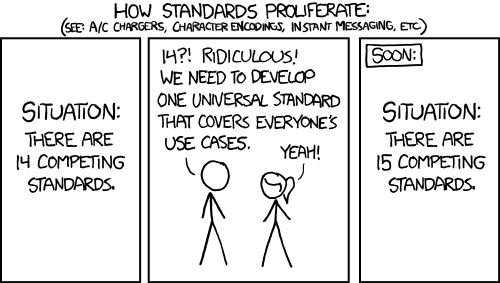
\includegraphics[width=.75\textwidth]{images/xkcd-standards}
	\caption*{\textit{Source: https://xkcd.com/927/\quad(CC BY-NC 2.5)}}
\end{figure*}

Simply put, the Dataflow Model aims to provide a unified way of thinking about data processing, producing a clear, composable abstraction.
It acknowledges the fact that it is impossible to design a perfect (always correct, low-latency and cheap) system, and instead it allows for tunability across these characteristics.

\Cref{sec:prep:dataflow} dives deep into the model itself and explains how these aims are achieved, while \cref{ch:impl} contains a detailed overview of the implementation of the model in practice.

\section{Why Elixir?}\label{sec:intro:elixir}

The Elixir language \cite{Elixir} is relatively young.
It is currently most popular in the web development circles, with many treating it as a Ruby replacement.
How then is this a suitable language in which to implement a robust, complex data processing system?

The answer lies in the underpinnings of the language.
Beneath the shiny, modern exterior lies the battle-hardened BEAM VM and OTP framework, which have been running Erlang-powered systems, mostly in the telecommunications industry, for decades.
We also have at our disposal the entire ecosystem of libraries written for Erlang.

Elixir is a dynamically typed, functional language with no variable mutability and with built-in support for efficiently managing and scheduling hundreds of thousands of \emph{processes} (akin to greenthreads) in a manner which is similar to the Calculus of Sequential Processes.
This invites the use of an actor-based model for applications, and indeed this is the standard approach in the Elixir/BEAM ecosystem.
These built-in primitives allow us to closely implement the desired semantics of the Dataflow Model without the overhead of thousands of lines of scheduling, threading and co\"ordinating\footnotemark[1] code (present in the existing Java implementation).

\footnotetext[1]{
For the typographically observant reader: the \"{} mark in ``co\"ordinating'' is a diaeresis---one of the two diacritical marks which are part of English natively (the other being the grave, as in ``the learn\`ed scholar'').
While its use is uncommon in modern English, some publications (notably The New Yorker) still employ it, and including it is the preferred style of the author.
It is used to indicate that two vowels should be pronounced separately, and not as a diphthong.
}

This project was completed using Elixir v1.4.2, and so all code examples and statements about the language apply to this version, the most current at the time of writing.
\Cref{sec:prep:elixir} gives a brief introduction to the language.



\section{Previous work}\label{sec:intro:previous}
Since the publication of the Dataflow paper \cite{Akidau:2015}, work has been ongoing to implement the Model in practice.
Initially, Google released the Google Cloud Dataflow product \cite{CloudDataflow} along with an SDK to allow users to easily construct data processing pipelines and run them on Google's cloud infrastructure.

In early 2016, Google decided to open-source the project and place it under the care of the Apache Foundation \cite{ApacheDataflowPost}.
This marked the beginning of Apache Beam, a project whose goals were even wider, and include support for cross-platform, cross-language compatibility through separating the creation of the pipelines and their execution on \emph{runners}.

The project has made excellent progress on these fronts, with a fully-featured SDK written in Java as well as a Python SDK.
It is compatible with many data processing systems such as Apache projects Spark, Storm and Flink.
Google Cloud Dataflow remains a paid product capable of running Beam pipelines at scale, but is now only one of many options for doing so.

The implementation also includes an on-machine local runner mainly aimed at testing workflows.
As the simplest yet fully-featured implementation of a Beam runner, it was used as the reference implementation for this project.

Several of the concepts introduced in the Dataflow paper have been used in other projects.
Notably, in the Elixir ecosystem, the Flow project \cite{ElixirFlow} takes some of the concepts---such as the windowing and triggering model---and provides a highly idiomatic way to write and execute multi-threaded computation in Elixir.
Its goals are, however, much narrower than the full Dataflow Model.

Flow has driven the development of GenStage \cite{ElixirGenStage}, a more low-level library implementing demand-driven data flow between actor processes, along with an extensible way to route, partition and dispatch that data.
GenStage forms the backbone of the execution logic in this project, and it is described in more detail in \cref{sec:todo}.

\section{Terminology}\label{sec:intro:terminology}

There are several similar and overloaded terms employed in this dissertation.
This section aims to clarify these and set a convention to be followed.
For a full list of defined terms, the reader should consult the <ref here to Appendix: Glossary>.

Due to the naming change to Apache Beam on open-sourcing the project, the reader will find various references to both the ``Dataflow`` and ``Beam`` on the web with little consistency.

The approach taken in this paper is to refer to the theoretical model described in \cite{Akidau:2015} as the Dataflow Model, and to the current, de facto official, implementation \cite{ApacheBeam} as Beam (generally referred to in full as Apache Beam).
Further, where the ``Beam Model'' is referenced, the author means the Dataflow extended with concepts now found in Apache Beam.
An overview of these is found in \cref{sec:impl:dataflow}.

The virtual machine which powers Erlang and Elixir is called the BEAM.
While efforts are made to refer to the conflicting software in full as the BEAM VM and Apache Beam, the reader should note that wherever the virtual machine is referred to, BEAM appears in all-uppercase form.

\section{Goals and focus}\label{sec:intro:goals}

At the outset, the goal of the project was to write an Elixir-based SDK in order to create Pipelines which could run on the existing Beam software.
Several weeks into the research it emerged concurrently that this approach was impractical to achieve, and that the front-end DSL itself was a relatively small task in itself, not suitable to form the entirety of the project.

The goal then shifted to writing an implementation of a subset of the Beam Model in Elixir.
However, due to the lack of explicit technical documentation of the Model, very quickly it emerged that in order to do this, a very significant amount of work had to be done to reverse-engineer it from an existing open-source codebase and community discussions.
As explained in \cref{sec:impl:dataflow}, many concepts have to be introduced in order to implement the Model, but they are not described directly in any reference material.

Therefore, a second goal of the project emerged, which proved to be a major focus---to extend and clarify the Dataflow Model with the concepts found in Apache Beam, such that a fuller, implementation-ready description is produced.
Once this work was completed, the initial goal of implementing this extended model was achieved with some additional effort.

\section{Results achieved}

Overall, the project was a success, in spite of proving much more challenging than originally imagined.
Due to the highly uncertain nature of the requirements, code had to be continually revisited and improved upon, and evaluation of progress was not straightforward.

Nevertheless, a working implementation of the Model was produced.
The implementation, while forgoing some features, delivered robust performance and a clean programmer interface, meshing well with existing language conventions.

A significant amount of currently non-existent documentation of the theory of the Beam Model was also produced, with some further extensions introduced which solve problems currently being tackled in the Beam Project.



\printbibliography

% Main document




\end{document}